\documentclass[journal,a4paper,comsoc,twocolumn]{IEEEtran}

\usepackage{amsmath,amsfonts,amssymb,amsthm,bm,mathtools}
\usepackage{algorithmic}
\usepackage{algorithm}
\usepackage{array}
\usepackage{tikz}
\usetikzlibrary{positioning,arrows.meta,fit}
\usepackage{textcomp}
\usepackage{stfloats}
\usepackage{url}
\usepackage{graphicx}
\usepackage{cite}
\usepackage{caption}
\usepackage{booktabs}
\usepackage[english]{babel}
\usepackage{enumitem}

\hyphenation{op-tical net-works semi-conduc-tor IEEE-Xplore}

\graphicspath{{Image/}{./}}  % also look beside main.tex if Image/ is missing

\renewcommand{\topfraction}{0.9}
\renewcommand{\bottomfraction}{0.8}
\renewcommand{\textfraction}{0.07}
\renewcommand{\floatpagefraction}{0.75}
\renewcommand{\dbltopfraction}{0.9}
\renewcommand{\dblfloatpagefraction}{0.75}

\newcommand{\Npop}{N_{\mathrm{pop}}}
\newcommand{\Ngen}{N_{\mathrm{gen}}}
% optional argument carries the subscript tail: \Ploss[,i] -> P_{loss,i}
\newcommand{\Ploss}[1][]{P_{\mathrm{loss}#1}}

\begin{document}
\raggedbottom

\title{A Two-Network Graph-Neural Pipeline for Delay-Constrained Multi-Link
EDCA Configuration in Wi-Fi~7}

\author{Vu Hoang Viet, Phan Van Thi%
\thanks{The authors are with the School of Information and Communications
Technology, Hanoi University of Science and Technology, Hanoi 100000, Vietnam.
% TODO: confirm affiliations and insert contact e-mail addresses before submission.
}%
}

\maketitle

\begin{abstract}
Configuring EDCA parameters across the links of a Wi-Fi~7 multi-link device
under per-category delay-violation constraints is currently solved by a genetic
search over an analytical delay model. Our results show that search
initialisation is the dominant bottleneck, while evaluation cost remains
substantial: on the reference five-category scenario, none of 600 sampled
configurations satisfies all five constraints simultaneously. We therefore
replace the expensive full genetic search with a pipeline of two graph neural
networks followed by lightweight refinement. A proposal network maps a scenario
directly to a population of candidate configurations, including the discrete
link assignment, and is trained
by the cross-entropy method with no solved instance as a label; an evaluation
network predicts the collision probability and delay-violation exponent, so
candidates are ranked without invoking the analytical model. One generation of
evolutionary refinement then polishes the proposal, and every reported value is
verified against the analytical model. Over 70 runs per method the genetic
baseline reaches the best observed objective in 4 and the proposed pipeline in
69 ($p = 1.6 \times 10^{-33}$), at 2.6~s and 142 analytical-model calls against
152.6~s and 29{,}309. Compared at equal compute rather than at equal search
settings, the ordering is strict: over twenty seeds the pipeline beats the
evaluation network alone, which beats the genetic baseline, at every one of the
40 wall-clock and 48 analytical-call budgets measured.
\end{abstract}

\begin{IEEEkeywords}
Wi-Fi~7, multi-link operation, EDCA, delay-bounded QoS, graph neural network,
learned proposal distribution, constrained configuration.
\end{IEEEkeywords}

\section{Introduction}
\label{sec:intro}

Multi-link operation (MLO) in IEEE~802.11be lets an access point multi-link
device (AP~MLD) place each traffic class on one of several links occupying
separate channels~\cite{Khorov2020,LopezPerez2019,LopezRaventos2022}. The EDCA
parameters --- contention window bounds, arbitration interframe space number,
transmission opportunity limit and retransmission limit --- must then be chosen
jointly with the link assignment, because categories sharing a link contend with
one another and categories on different links do not.

Yi \emph{et al.}~\cite{Yi2025} pose this as maximising delivery reliability
subject to a delay-violation probability constraint per access category and
solve it with a genetic algorithm (GA) whose fitness function is an analytical
model of the EDCA delay distribution. We adopt that formulation. Its cost is
dominated by the fitness function: one evaluation needs a fixed point of a
collision-probability recursion per link and a numerical
generating-function inversion per category, taking $16$~ms on one core in our
implementation, and the configuration of~\cite[Table~I]{Yi2025} corresponds to
about $10^{6}$ evaluations per run.

The obvious response is to make evaluations cheaper. We implemented that first,
and the outcome redirected the work: a surrogate reproducing the fitness ranking
at Spearman $\rho = 0.9996$, cutting exact evaluations by $19.8\times$, left
solution quality statistically unchanged --- 8 successful runs in 70 against 4
for the baseline ($p = 0.37$). Cheaper evaluation is worth having --- at a
matched compute budget it beats the baseline at every point we measured
(Section~\ref{sec:cost}) --- but it does not by itself change how often a run
succeeds.

Section~\ref{sec:hard} identifies what does. On the five-category scenario
of~\cite[Sec.~V]{Yi2025}, 300 configurations drawn uniformly from the parameter
domain and 300 drawn from a hand-designed structured region contain no feasible
point at all; even perturbations of the optimum are feasible only $1.5\%$ of the
time. A search starting from any of those distributions spends its budget
crossing the infeasible region, and making each evaluation cheaper shortens
that crossing without removing it. A better proposal distribution removes
it.

Our contributions are as follows.

\begin{itemize}[leftmargin=*,itemsep=1pt,topsep=2pt]
\item We quantify the geometry that governs the problem
(Section~\ref{sec:hard}): the joint feasibility rate is below the resolution of
600 samples, while per-category rates in the structured region are $4$, $5$,
$25$, $90$ and $98\%$. The difficulty is the conjunction, not any one
constraint.
\item We propose a two-network pipeline (Section~\ref{sec:pipe}) in which a
graph network proposes configurations and a second graph network ranks them,
with the architecture read off the fixed-point recursion rather than chosen by
analogy. Neither network requires a solved instance as a label.
\item We show that, under the evaluated settings, one generation of
refinement captures nearly all of the attainable gain, and report a $10/10$
success rate at $2.6$~s and $142$ analytical-model calls
against $1/10$, $152.6$~s and $29{,}309$ calls for the baseline
(Section~\ref{sec:results}).
\end{itemize}

\section{Related Work}
\label{sec:related}

The delay model used here descends from Bianchi's mean-value
analysis~\cite{Bianchi2000} through the extensions that added service
differentiation: Kong \emph{et al.}~\cite{Kong2004} and Xiao~\cite{Xiao2005}
analyse the IEEE~802.11e priority mechanisms, and Inan \emph{et
al.}~\cite{Inan2009} derive the AIFS zone decomposition on which
Section~\ref{sec:system} rests. Those analyses report throughput and mean
delay, whereas the constraint treated here is a tail probability as small as
$10^{-7}$ and needs the whole delay distribution, obtained
in~\cite{Yi2025} by numerical inversion~\cite{AbateWhitt1992}. Work on MLO
itself has mainly quantified the gain the feature
offers~\cite{LopezRaventos2022,Naik2021} rather than producing the parameter
assignment that realises it.

Learning has been applied across the IEEE~802.11 stack~\cite{Szott2022}. The
nearest strand tunes contention windows online by reinforcement learning:
Wydma\'{n}ski and Szott~\cite{Wydmanski2021} adapt a single window in
IEEE~802.11ax against a throughput reward, and Liu \emph{et al.}~\cite{Liu2026}
jointly learn traffic allocation and initial window sizes for Wi-Fi~7 MLO. Both
optimise throughput from interaction with a running network; the present problem
is a one-shot configuration of six parameters per category under hard
constraints on a tail no feasible amount of interaction would estimate at
$10^{-7}$, so our training signal comes from the analytical model instead.

Graph networks are used for radio resource allocation because the permutation
equivariance of message passing~\cite{Gilmer2017} matches the symmetry of an
interference graph~\cite{Shen2021,Eisen2020,Sun2018}; there the graph is fixed
by the channel gains, whereas here it is the link assignment and is itself
decided. Screening an expensive fitness function with a cheap model is standard
in surrogate-assisted evolutionary computation~\cite{Jin2011}; our finding is
that in this problem evaluation acceleration alone improves efficiency but does
not address poor initialisation, and that the same network class applied to the
\emph{proposal} is what changes the outcome. The proposal
network can also be used without any search, which we study
separately~\cite{Companion}.

\section{System Model and Problem Formulation}
\label{sec:system}

An AP~MLD operates $M$ links and carries $I$ access categories indexed by
$i \in \mathcal{I}$ (Fig.~\ref{fig:system}). Category $i$ is offered by $n_i$
saturated stations sending $L_i$-byte payloads and must satisfy
\begin{equation}
\label{eq:qos}
\Pr(D_i \ge D_{\max,i}) < \varepsilon_i ,
\end{equation}
with $D_i$ the head-of-queue-to-acknowledgement delay, $D_{\max,i}$ the budget
and $\varepsilon_i$ the tolerated violation probability. Links occupy separate
channels and are analysed independently. The decision variables are
\begin{equation}
\label{eq:decision}
\mathbf{x}_i = (CW_{\min,i},\, CW_{\max,i},\, AIFSN_i,\, TXOP_i,\, R_i,\, m_i),
\end{equation}
with $CW_{\min,i} \le CW_{\max,i}$ in $[1,1023]$, $AIFSN_i \in [2,15]$,
$TXOP_i \in [0,8192]\,\mu$s in $32\,\mu$s steps, $R_i \in [4,7]$, and $m_i$ the
link index. Including $m_i$ is what distinguishes the MLO problem from
single-link EDCA tuning.

\begin{figure}[!t]
\centering
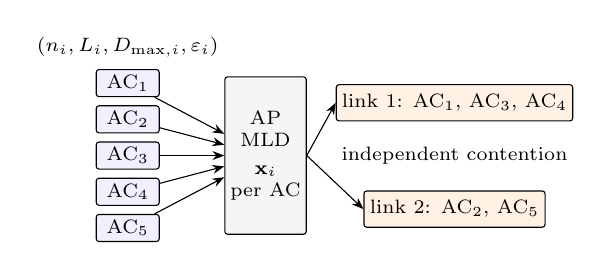
\begin{tikzpicture}[
  font=\scriptsize,
  box/.style={draw,rounded corners=1pt,inner sep=2pt,align=center},
  ac/.style={box,fill=blue!6,minimum width=8mm,minimum height=3.4mm},
  lk/.style={box,fill=orange!10,minimum width=23mm,minimum height=4.6mm},
  >={Stealth[length=1.5mm]}]
\node[ac] (a1) at (0,0)      {AC$_1$};
\node[ac] (a2) at (0,-0.46)  {AC$_2$};
\node[ac] (a3) at (0,-0.92)  {AC$_3$};
\node[ac] (a4) at (0,-1.38)  {AC$_4$};
\node[ac] (a5) at (0,-1.84)  {AC$_5$};
\node at (0,0.46) {$(n_i,L_i,D_{\max,i},\varepsilon_i)$};
\node[box,fill=gray!8,minimum height=20mm,minimum width=9mm]
      (mld) at (1.75,-0.92) {AP\\MLD\\[2pt]$\mathbf{x}_i$\\per AC};
\node[lk] (l1) at (4.15,-0.25) {link $1$: AC$_1$, AC$_3$, AC$_4$};
\node[lk] (l2) at (4.15,-1.60) {link $2$: AC$_2$, AC$_5$};
\node at (4.15,-0.92) {independent contention};
\foreach \a in {a1,a2,a3,a4,a5} \draw[->] (\a) -- (mld);
\draw[->] (mld.east) -- (l1.west);
\draw[->] (mld.east) -- (l2.west);
\end{tikzpicture}
\caption{The AP~MLD selects one parameter vector $\mathbf{x}_i$ per access
category, including the link on which that category contends. Categories on a
shared link contend; the links use separate channels. The assignment shown is
the one returned in Section~\ref{sec:results}.}
\label{fig:system}
\end{figure}

Categories with different $AIFS_i$ become eligible to decrement their backoff
counters at different instants, so the timeline splits into zones, zone $j$
collecting slots whose eligible set $Z_j$ is the same. With $p_k$ the per-slot
transmission probability of category $k$ and $r_k = 1-p_k$, a slot of zone $j$
is idle with probability $q_j = \prod_{k \in Z_j} r_k^{\,n_k}$, and the
collision probability is the zone average
\begin{equation}
\label{eq:ck}
c_k = \sum_{j \ge Z_k^0} \frac{\pi_j}{\sum_{j' \ge Z_k^0}\pi_{j'}}
      \left(1 - \frac{q_j}{r_k}\right),
\end{equation}
with $\pi_j$ the stationary probability of zone $j$ and $Z_k^0$ the first zone
in which $k$ is eligible. Together with a mean-value expression for
$p_k$~\cite{Bianchi2000} this forms a fixed point solved per link by damped
iteration, giving $\Ploss[,k] = c_k^{\,R_k}$. The reliability index
$\theta_k = -\log_{10}\Pr(D_k \ge D_{\max,k})$ follows by Fourier-series
inversion~\cite{AbateWhitt1992} of the delay generating function
of~\cite[Eqs.~(10)--(15)]{Yi2025}. The design problem is
\begin{equation}
\label{eq:P1}
\max_{\{\mathbf{x}_i\}} \; F = \sum_{i\in\mathcal{I}} -\log_{10} \Ploss[,i]
\quad \text{s.t.} \quad \eqref{eq:qos},\; \mathbf{x}_i \in \mathcal{X} .
\end{equation}
We clip $\Ploss[,i]$ at $10^{-10}$, which is both the axis floor
of~\cite{Yi2025} and the resolution of the model, so each category contributes
at most $10$ and the five-category scenario has a ceiling of $F = 50$.
Candidates are ranked by $F$ when feasible and by
$-\tfrac{1}{2}\sum_i u_i$ otherwise, where
$u_i = [\log_{10}(\Pr(D_i \ge D_{\max,i})/\varepsilon_i)]^{+}$ counts the
decades of excess.

\section{Structure of the Search Problem}
\label{sec:hard}

Two properties of~\eqref{eq:P1} determine how a solver should spend its budget,
and they call for different remedies. Table~\ref{tab:scenario} gives the
scenario throughout.

\begin{table}[!t]
\centering
\caption{Five-category evaluation scenario~\cite[Sec.~V]{Yi2025}.}
\label{tab:scenario}
\small
\setlength{\tabcolsep}{4pt}
\begin{tabular}{lccccc}
\toprule
 & AC$_1$ & AC$_2$ & AC$_3$ & AC$_4$ & AC$_5$ \\
\midrule
Stations $n_i$            & $2$ & $4$ & $4$ & $3$ & $3$ \\
Payload $L_i$ (B)         & $50$ & $210$ & $256$ & $800$ & $2000$ \\
Budget $D_{\max,i}$ (ms)  & $50$ & $60$ & $100$ & $300$ & $300$ \\
Threshold $\varepsilon_i$ & $10^{-7}$ & $10^{-6}$ & $10^{-4}$ & $10^{-2}$ & $0.5$ \\
\bottomrule
\end{tabular}
\end{table}

The first is evaluation cost: $16$~ms per call, so a run at $\Npop = 200$ over
$\Ngen = 300$ generations consumes about $2.9\times10^{4}$ calls and $153$~s in
median. This argues for a cheap approximate ranking.

The second is the measure of the feasible set, and it is the one that governs
the outcome. Uniform sampling over $\mathcal{X}$ produces no feasible
configuration in $300$ draws. Sampling from a structured region --- large
contention windows, narrow window span, $R_i = 7$, background categories at
large $AIFSN$ --- also produces none, although its per-category rates are $4$,
$5$, $25$, $90$ and $98\%$: the two categories carrying the tight thresholds are
satisfied a few percent of the time and feasibility needs all five at once. Even
Gaussian perturbations of the optimum with relative standard deviation $0.15$
land inside only $1.5\%$ of the time.

A population drawn from any of these begins with no feasible individual, so a
search must first cross the infeasible region under the penalty term. Making
each evaluation cheaper accelerates that crossing but does not remove it. The
pipeline of Section~\ref{sec:pipe} addresses both properties, with one network
for each.

\section{The Graph-Neural Pipeline}
\label{sec:pipe}

The method is
\begin{equation}
\label{eq:pipeline}
\text{scenario}
\;\xrightarrow{\;\pi_\psi\;}\; \text{population}
\;\xrightarrow{\;g_\phi\;}\; \text{ranking}
\;\xrightarrow{\;\text{1 gen.}\;}\; \text{polish}
\;\xrightarrow{\;f\;}\; \text{verified,}
\end{equation}
where $\pi_\psi$ proposes, $g_\phi$ ranks, and $f$ is the analytical model,
which is called only on the few candidates that survive screening and always on
the incumbent, so no reported value is ever a prediction.

\subsection{Graph Representation}

Taking the logarithm of the idle-slot product gives
$\log q_j = \sum_{k \in Z_j} n_k \log r_k$, a permutation-invariant sum over
contending categories with $n_k$ as an edge weight and $\log r_k$ as a message;
the $\pi_j$-weighted average in~\eqref{eq:ck} is a second aggregation. The
damped iteration that solves the fixed point therefore applies one aggregation
operator repeatedly, which is message passing~\cite{Gilmer2017} with weights
shared across rounds. This fixes three choices that a multilayer perceptron
would leave open: permutation invariance over categories is structural, one
network serves scenarios with different numbers of categories, and the link
assignment becomes the \emph{topology} rather than one more input feature.

For $g_\phi$, each category is a node and nodes $i,j$ are joined iff
$m_i = m_j$, so the adjacency matrix is the link assignment. Node features are
the scenario descriptors, the decision variables and the closed-form
transmission durations; edge features are $n_j$, the AIFS offset and two
zone-overlap indicators. Quantities that already have closed forms are supplied
rather than learned. Graphs have $3$ to $8$ nodes, so dense adjacency matrices
are used. For $\pi_\psi$ the graph is instead complete over the categories,
since the link assignment is an output and cannot also define the adjacency.

\subsection{Proposal Network}
\label{sec:propose}

$\pi_\psi$ maps a scenario to a distribution over the discrete levels of every
gene, including the link index, and the population is drawn from it. Node
features add the relative rank of $\varepsilon_i$ and $D_{\max,i}$ among the
categories present, because what determines a good configuration is mainly which
category is tighter than which. It replaces a set of manual seeding rules that
encode real structure but are the same for every scenario and, as
Section~\ref{sec:hard} records, still yield nothing feasible in $300$ draws.

Training uses the cross-entropy method~\cite{DeBoer2005} with no solved
instance as a label: each step, $\pi_\psi$ proposes $K = 96$ configurations for
each of $32$ scenarios, $g_\phi$ scores all $3{,}072$ in one forward pass, the
best $12.5\%$ form the elite set, and $\pi_\psi$ is updated towards it. Only the
\emph{ranking} is needed, which is what $g_\phi$ supplies most reliably, and
scoring $3{,}072$ configurations costs $15$~ms against $49$~s with the
analytical model. Training runs $1500$ steps in $81$~s. At solve time the
population is drawn in one batch --- one greedy sample plus the rest at
temperature $1.6$, since a converged policy is nearly deterministic --- and
ranked by $g_\phi$, costing $8.4$~ms.

\subsection{Evaluation Network}
\label{sec:evaluate}

$g_\phi$ predicts $(\log_{10} c_i, \theta_i)$ per category. It applies $T = 6$
weight-shared rounds of
\begin{equation}
\label{eq:mp}
h_i \leftarrow h_i + \mathrm{Upd}\Big(\big[h_i,\;
  \textstyle\sum_j A_{ij} m_{ij} \,\|\, \max_j A_{ij} m_{ij}\big]\Big),
\end{equation}
with $m_{ij} = \mathrm{Msg}([h_i, h_j, e_{ij}])$. Aggregation is a sum because
$\log q_j$ is a sum and a mean would normalise away how many stations contend;
weights are shared because the analytical solver applies one operator
repeatedly, so $T$ rounds emulate $T$ \emph{iterations}, not $T$ hops; the
residual makes one round an increment. The network predicts $\log_{10} c_i$
rather than $\Ploss[,i]$, since $F$ is linear in it once
$\Ploss[,i] = c_i^{R_i}$ is applied exactly afterwards, so the exponentiation
that amplifies error is never learned; and $\theta_i$ rather than the raw
probability, whose dynamic range at $10^{-7}$ is unusable. The model has
$156{,}386$ parameters.

Labels come from the analytical model, so data is limited only by compute, but
Section~\ref{sec:hard} makes the sampling distribution the difficulty. We
therefore log GA trajectories: every configuration a GA evaluates has already
passed through the analytical model, so recording it adds no evaluations and the
distribution matches the one $g_\phi$ will face. Mixing $45\%$ trajectory with
$55\%$ broad sampling gives $200{,}000$ samples of which $8.19\%$ are feasible
and $19.10\%$ lie within one decade of a boundary, against $0\%$ for uniform
sampling; generation takes $159$~s on $26$ cores and training $387$~s.

On $20{,}000$ held-out samples the RMSE of $\log_{10} c$ is $0.0108$ and of
$\theta$ is $0.393$, with Spearman $\rho = 0.9996$ on the fitness and $99.19\%$
feasibility-decision accuracy. On the $3{,}778$ near-boundary samples --- the
regime that decides screening --- $\rho$ is $0.9824$ and accuracy $95.74\%$. An
RMSE of $0.393$ on $\theta$ is a factor of $2.47$ in probability, the same order
as the gap between the analytical model and slot-level simulation, so $g_\phi$
is about as accurate as the quantity it approximates.

\subsection{Refinement}
\label{sec:refine}

Each generation, $g_\phi$ scores the population in one forward pass and only the
$V = 8$ most promising individuals reach the analytical model. Coordinate
refinement is screened the same way: $g_\phi$ scores every level of a gene in
one call and only the three best are evaluated exactly, which is cheaper than an
unscreened sweep and searches more, since it examines all levels rather than a
$\pm 2$ neighbourhood. How many generations are needed is an empirical question,
answered in Section~\ref{sec:results}: one.

\section{Numerical Results}
\label{sec:results}

All methods share the population grid $\Npop \in \{6,\dots,200\}$, the same
generation and stagnation budgets and the same ten seeds, giving $70$ runs each.
Every objective value is computed by the analytical model. A run is a
\emph{success} if it reaches within $1\%$ of the best value observed anywhere in
the study ($F \ge 49.21$), one threshold for all methods. Timings are on one
RTX~4060 and a 26-core CPU. Three configurations recur and are cumulative: the
genetic baseline, the baseline with $g_\phi$ screening its candidates, and that
with $\pi_\psi$ also seeding its population.

One convention matters for reading the results together. The baseline's
objective is not one number: it runs here at $3{,}362$, $13{,}105$ and
$29{,}309$ analytical-model calls, and its outcome on a single run is besides
strongly bimodal, so any ten-seed summary of it moves by several objective
points between seed sets. Every figure therefore states the budget and the
statistic it reports, and Table~\ref{tab:cost} gives the trajectory against
budget that the figures are readings from. Where one run is compared with one
run we report medians and not best-of-$N$, which has $N$ chances where one run
has one.

\begin{figure*}[!t]
\centering
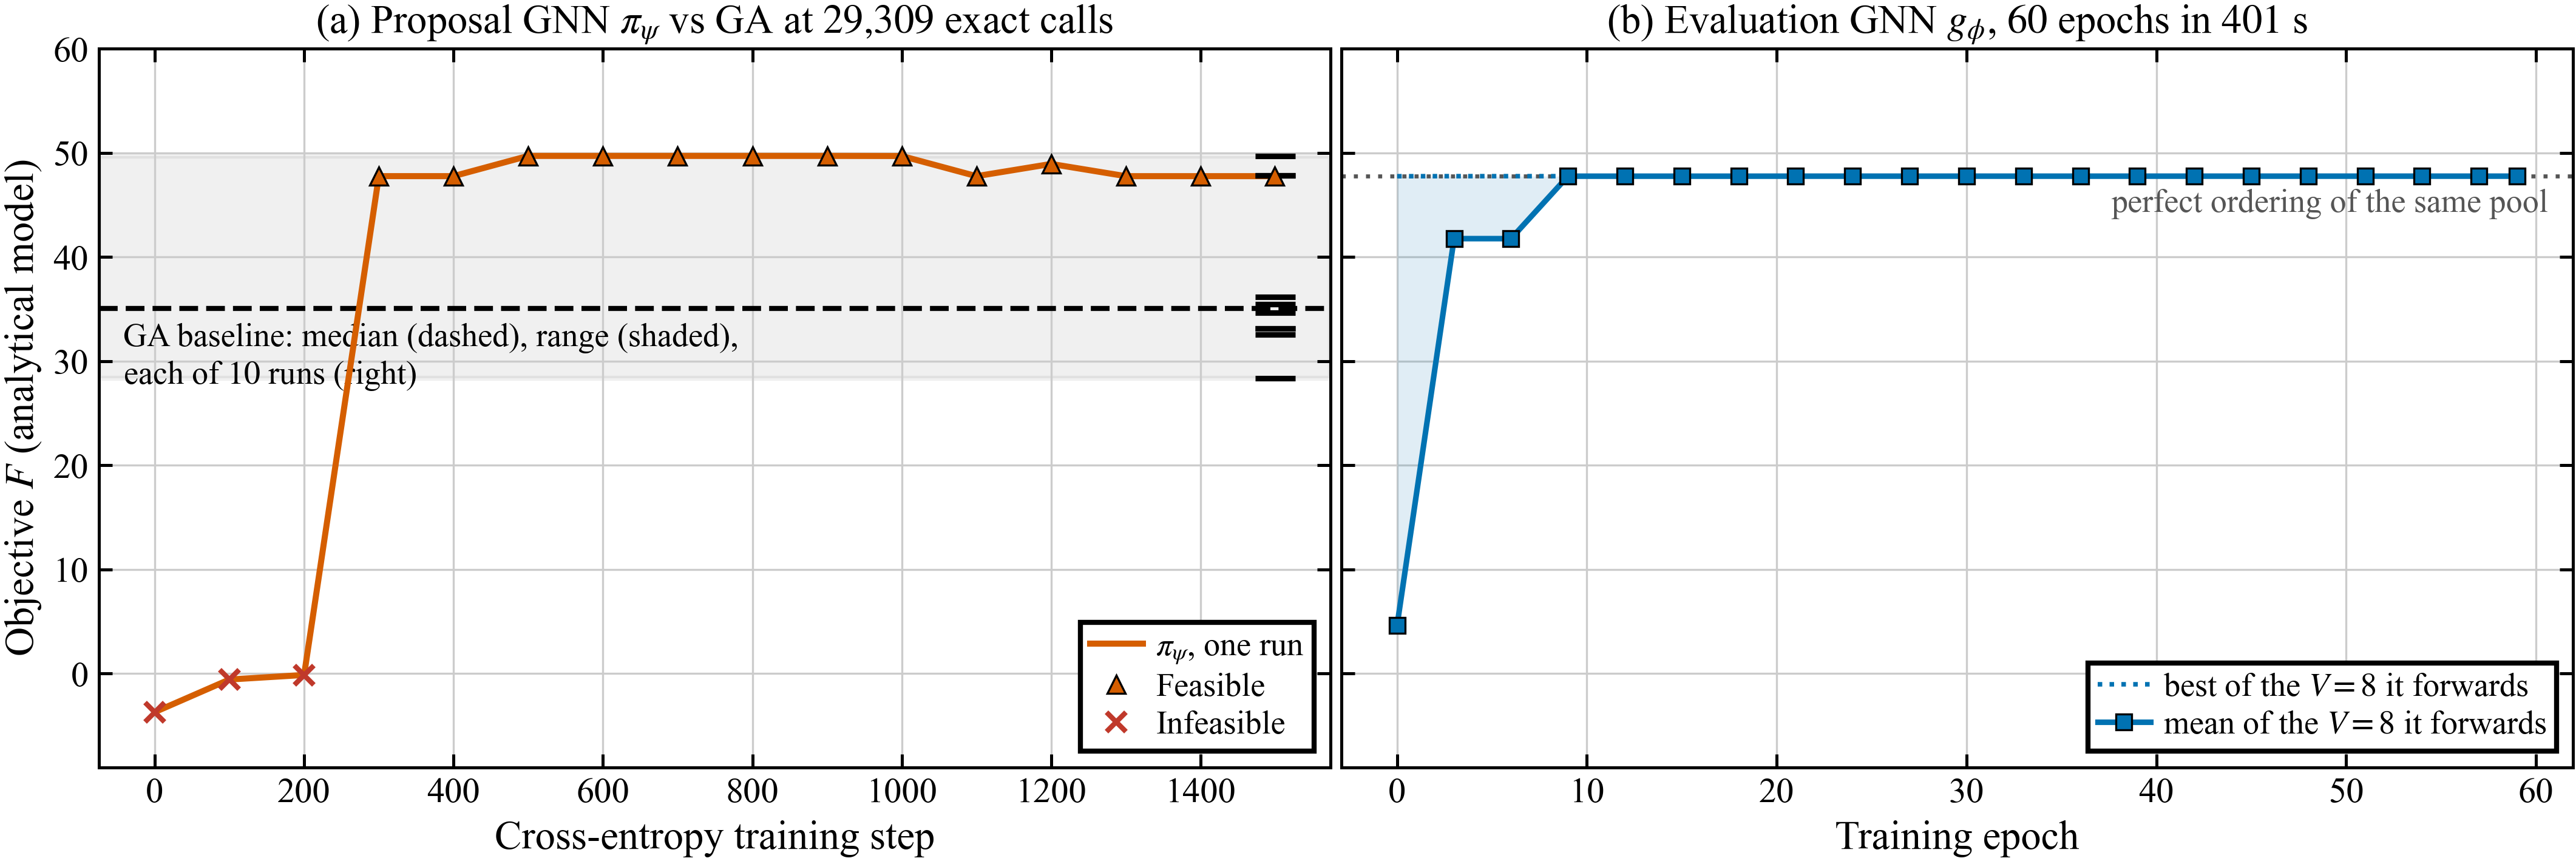
\includegraphics[width=\textwidth]{fig10_gnn_training.png}
\caption{Training convergence of both networks. They are trained on different
problems and cannot share an $x$ axis, but they share the $y$ axis: each is
scored by the objective its own output achieves under the analytical model.
(a) $\pi_\psi$ emits a configuration, scored by that configuration's exact $F$,
against the baseline at $29{,}309$ exact calls per run: median dashed, range
shaded, the ten runs drawn at the right edge. Not their best --- one run is
compared with one run, and seven of the ten fall below what the network
returns. (b) $g_\phi$ emits an \emph{ordering}, so it is scored as the pipeline
uses it --- the mean exact $F$ of the $V = 8$ candidates it forwards, from a
pool of $1{,}560$ configurations scored once in advance. A regression error does
not belong on this axis; the ranking it induces does.}
\label{fig:train}
\end{figure*}

\subsection{Convergence of the Two Networks}

Fig.~\ref{fig:train} scores each network by what its own output achieves rather
than by its training loss, the two losses sharing neither units nor meaning; the
ordering $g_\phi$ emits is scored as the pipeline uses it. They converge at very
different points in their budgets. $\pi_\psi$ produces its first feasible
configuration at step $300$, crossing the baseline's median there, and settles
at $47.76$ --- above seven of the ten baseline runs, each of which costs
$29{,}309$ exact calls against the $8.4$~ms this network needs to draw a
population once trained. Training to that point takes $27$~s of the $81$~s
total. $g_\phi$ reaches an ordering within $0.1\%$ of a perfect one after $9$ of
$60$ epochs, and the remaining $51$ move it no further. Ranking configurations
is the easier problem, and Section~\ref{sec:cost} shows that solving it well is
also worth less.

\begin{figure*}[!t]
\centering
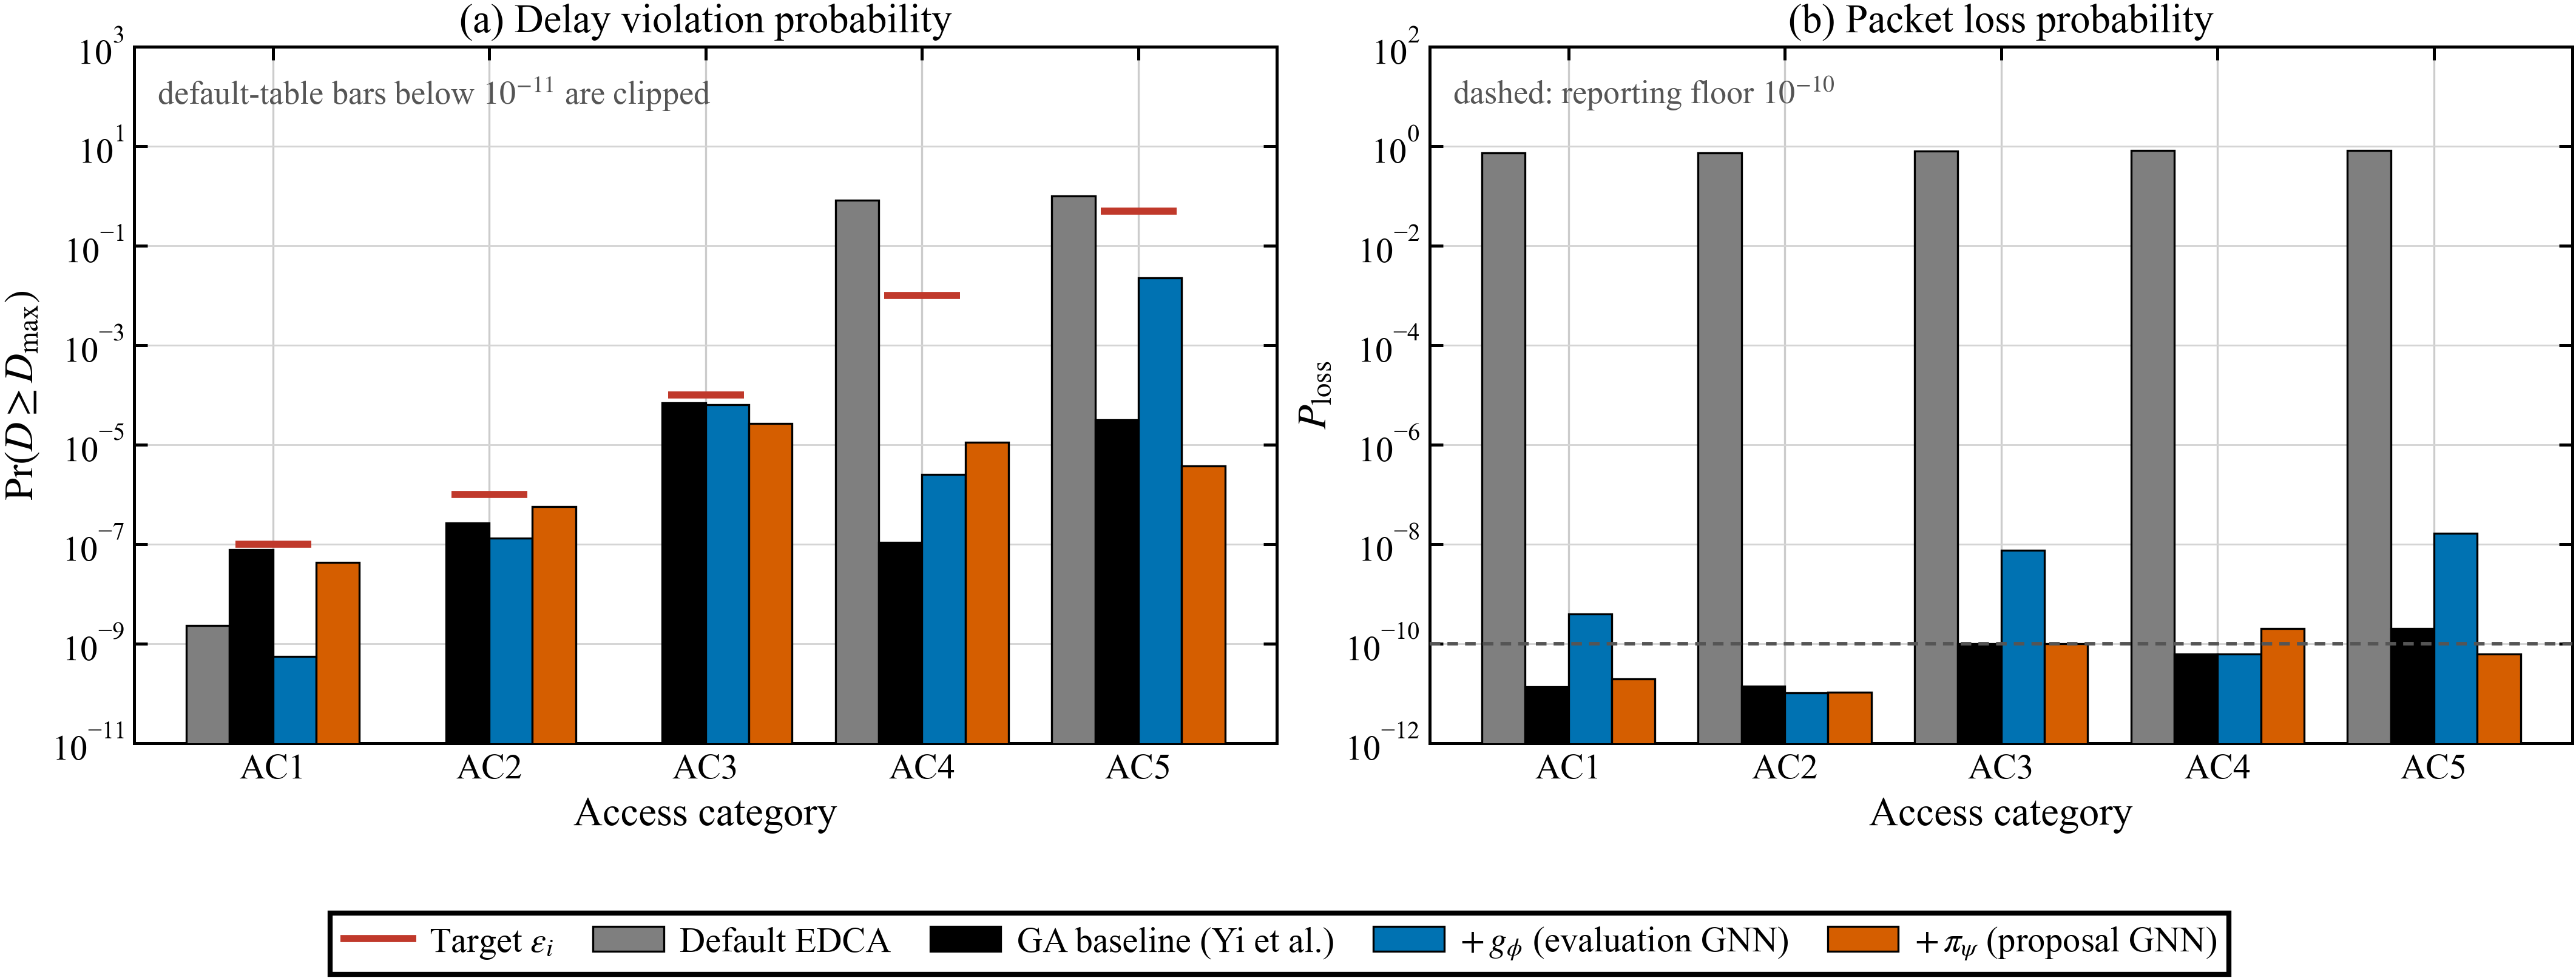
\includegraphics[width=\textwidth]{fig09_qos_methods.png}
\caption{Per-category QoS of the returned configuration: (a) delay-violation
probability against the target $\varepsilon_i$, (b) packet-loss probability.
Each method is shown at its best of ten restarts at $\Npop = \Ngen = 120$,
because on this scenario the spread between restarts is wider than the spread
between methods; that budget costs the baseline $13{,}105$ exact calls, which is
why its objective here exceeds the one in Fig.~\ref{fig:sweep}. The default
table violates AC$_4$ and AC$_5$; all three optimised configurations satisfy
every constraint, and the two that include $\pi_\psi$ also sit on the $\Ploss$
reporting floor.}
\label{fig:qos}
\end{figure*}

\subsection{Correctness of the Returned Configuration}

Fig.~\ref{fig:qos} compares the default IEEE~802.11e table against all three
optimised configurations. The default table violates AC$_4$ and AC$_5$ by
roughly two orders of magnitude and loses $73$--$83\%$ of packets in every
category. All three optimised configurations satisfy all five constraints, so
panel~(a) shows that optimisation is necessary without distinguishing the
optimisers. Panel~(b) distinguishes them, and only because the
screened-but-unseeded configuration is present: it leaves $\Ploss$ at
$7.6\times10^{-9}$ on AC$_3$ and $1.6\times10^{-8}$ on AC$_5$, two to three
decades above the baseline and the full pipeline, which both sit on the
$10^{-10}$ floor. Screening the fitness evaluation buys speed, not solution
quality; the margin comes from the seeding.

\begin{figure*}[!t]
\centering
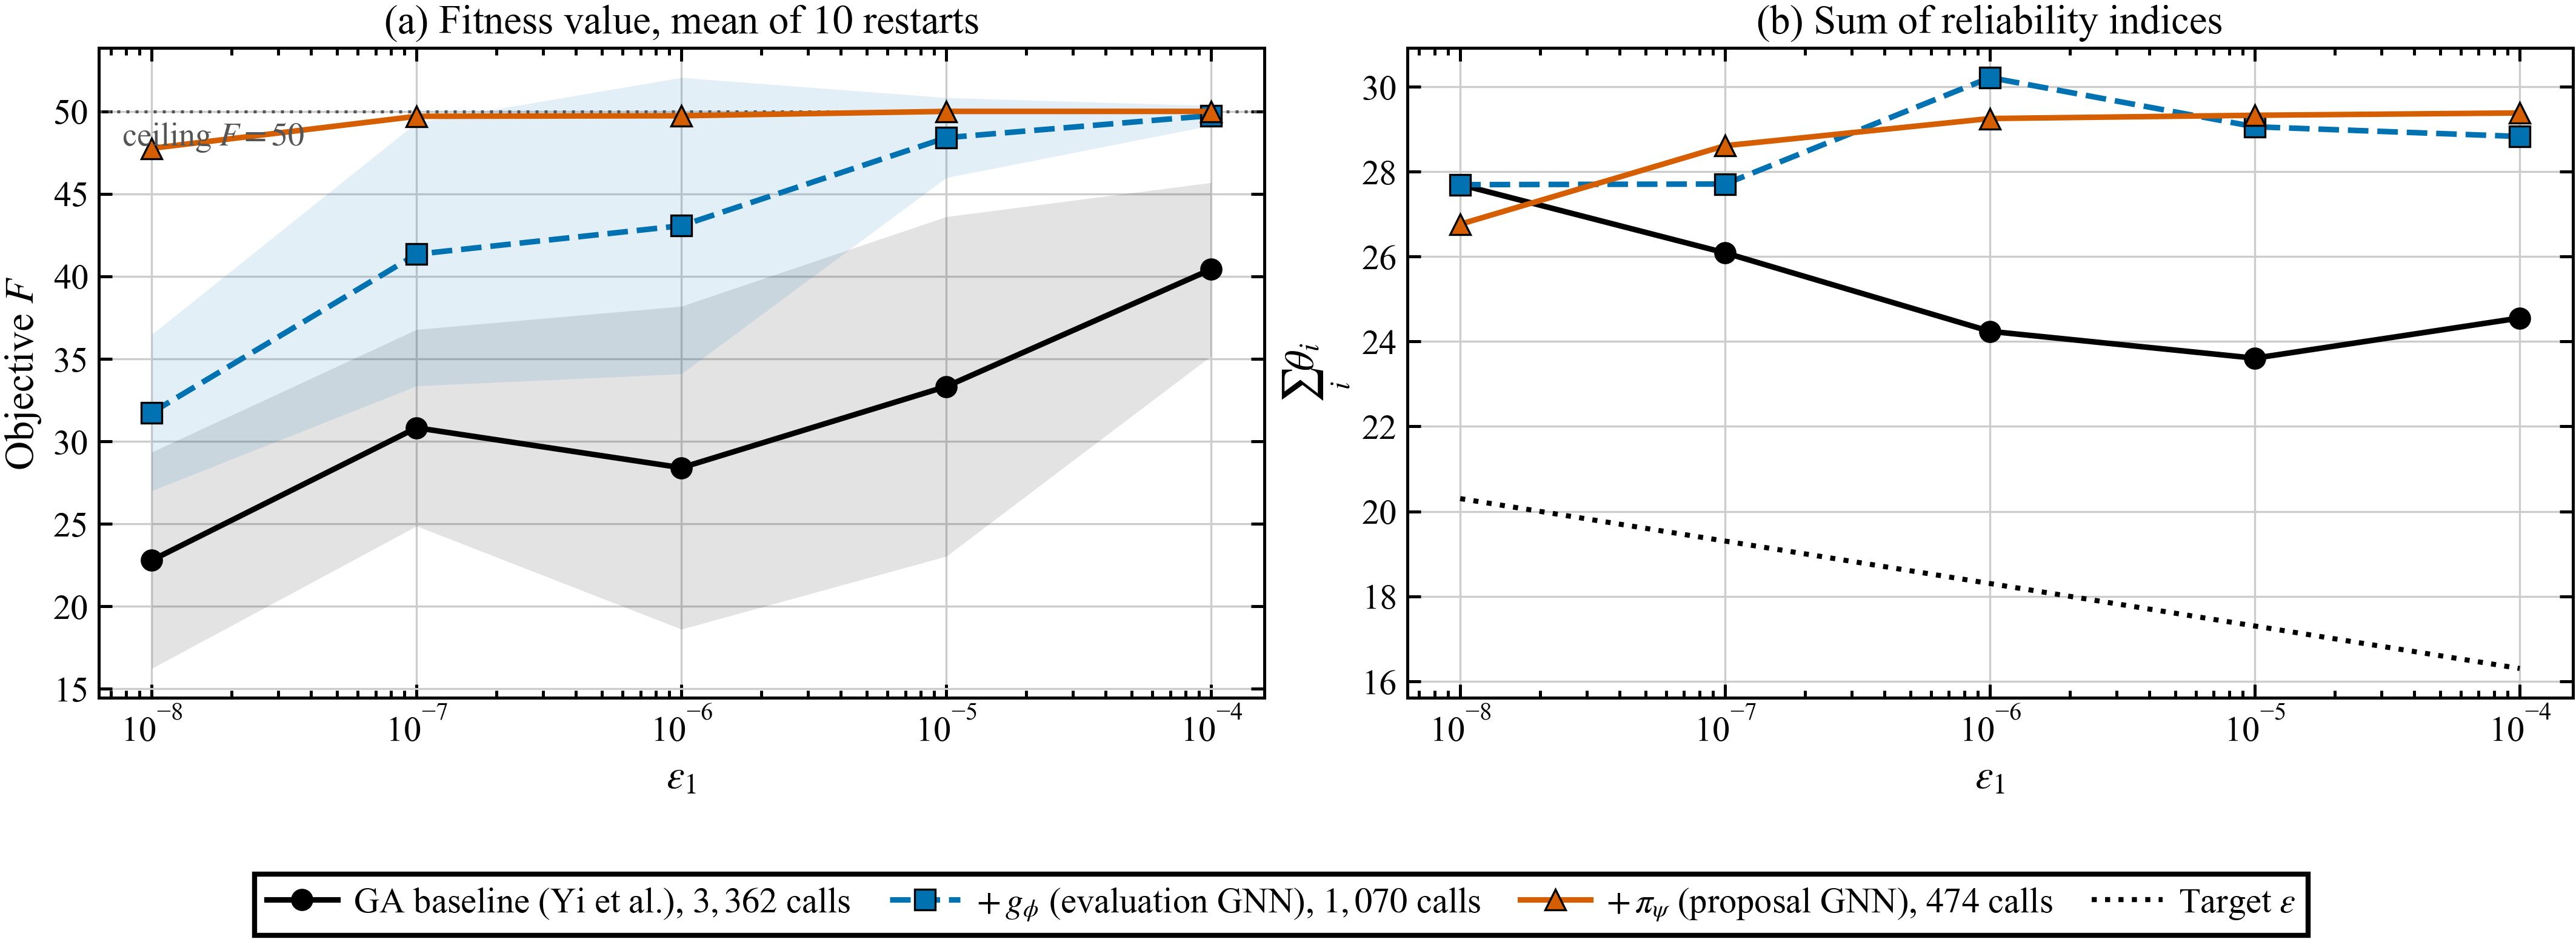
\includegraphics[width=\textwidth]{fig08_sweep_methods.png}
\caption{Behaviour when the tightest threshold moves: (a) objective, (b) sum of
reliability indices, against $\varepsilon_1$ over five decades. The baseline
runs at the configuration that reproduces the objective reported for it
in~\cite{Yi2025}; each network runs at the largest configuration we measured
and, even so, spends fewer exact calls than the baseline --- $1{,}065$ and
$478$ against $3{,}362$, as the legend records --- because screening makes each
candidate cheaper. Each curve is the \emph{mean} over forty restarts, shaded by
one standard deviation in (a). The band is itself a result: the pipeline's
deviation never exceeds $0.12$, so its mean is its outcome, while the unseeded
methods scatter by up to $8.7$ points. A mean is not bounded by the monotonicity
of $F^\star$, which constrains the optimum rather than the solver's output
distribution.}
\label{fig:sweep}
\end{figure*}

\subsection{Robustness to the Threshold}

Fig.~\ref{fig:sweep} repeats the comparison across five decades of
$\varepsilon_1$, forty restarts per point. The baseline is run at the search
configuration that reproduces the objective reported for it in~\cite{Yi2025},
about $35$ at $\varepsilon_1 = 10^{-4}$; ours reaches $40.55$ there, the closest
point on our grid and slightly in its favour. Each network is then given the
largest configuration we measured, which still costs it $1{,}065$ and $478$
exact calls against the baseline's $3{,}362$ --- $3.2\times$ and $7.0\times$
fewer --- because a screened candidate is cheaper than an exactly evaluated one.
The sweep also admits a monotonicity check: the objective~\eqref{eq:P1} does not
contain $\varepsilon$, which enters only through~\eqref{eq:qos}, so relaxing
$\varepsilon_1$ enlarges the feasible set without changing what is maximised
over it and $F^\star$ cannot fall. That bound is on the optimum, not on the mean
plotted here, which is non-decreasing for all three regardless. The baseline
averages $25.43$ at $\varepsilon_1 = 10^{-8}$ rising to $40.55$ at $10^{-4}$,
the evaluation network $31.89$ to $49.92$ and the pipeline $47.76 \pm 0.00$ to
$50.00 \pm 0.00$: the ordering $\pi_\psi > g_\phi > \text{baseline}$ holds at
all five thresholds while the call counts run the other way, on five scenarios
rather than one, which partly addresses the limitation in
Section~\ref{sec:limits}.

\begin{table}[!t]
\centering
\caption{Cost and quality. \textbf{Top:} at one search configuration
($\Npop = 200$, $\Ngen = 300$), medians over $10$ seeds; the last row is the
pipeline at the refinement depth measured to be sufficient. ``Feas.\ init.'' is
the fraction of the initial population already feasible. \textbf{Bottom:} mean
objective over $20$ seeds at a shared wall-clock budget, no early stopping.
Exact calls are machine independent; wall-clock time is not. Training is paid
once for all scenarios: $159$~s for the training set, $401$~s for $g_\phi$,
$81$~s for $\pi_\psi$.}
\label{tab:cost}
\small
\setlength{\tabcolsep}{3pt}
\begin{tabular}{lccccc}
\toprule
Configuration & Time (s) & Exact calls & $F$ & Success & Feas.\ init. \\
\midrule
GA baseline~\cite{Yi2025} & $152.6$ & $29{,}309$ & $35.04$ & $1/10$ & $0\%$ \\
\;\; $+$ evaluation GNN $g_\phi$ & $32.2$ & $1{,}483$ & $34.63$ & $2/10$ & $0\%$ \\
\;\; $+$ proposal GNN $\pi_\psi$ & $13.6$ & $607$ & $49.70$ & $10/10$ & $33\%$ \\
\midrule
Pipeline, $\Ngen = 1$ & $2.6$ & $142$ & $49.70$ & $10/10$ & $33\%$ \\
\bottomrule
\end{tabular}

\vspace{2pt}

\begin{tabular}{lccc}
\toprule
Budget (s) & GA baseline & $+\,g_\phi$ & $+\,g_\phi+\pi_\psi$ \\
\midrule
$0.99$ & --- & $13.77$ & $49.69$ \\
$2.9$ & $0.48$ & $21.46$ & $49.69$ \\
$9.8$ & $14.97$ & $32.80$ & $49.69$ \\
$29$ & $23.38$ & $42.46$ & $49.70$ \\
$97$ & $34.64$ & $43.01$ & $49.70$ \\
$250$ & $41.69$ & $43.01$ & $49.70$ \\
\bottomrule
\end{tabular}
\end{table}

\subsection{Cost and Quality under a Common Budget}
\label{sec:cost}

The top of Table~\ref{tab:cost} fixes the search configuration and varies only
which networks are present. On that comparison $g_\phi$ is not expected to raise
the objective: it replaces an exact evaluator with an approximate one, so at an
equal number of candidates examined it can at best match the baseline, and it
carries prediction error besides. It does exactly that --- $34.63$ against
$35.04$ --- while cutting exact calls by $19.8\times$ and time by $4.7\times$,
and it moves the success rate only from $4/70$ to $8/70$ across the full grid,
which a two-sided Fisher exact test places at $p = 0.37$. Adding $\pi_\psi$
moves that rate to $69/70$, $p = 1.6\times10^{-33}$ against the baseline and
$2.8\times10^{-29}$ against $g_\phi$ alone; because $g_\phi$ is held fixed
across those rows, the gain is attributable to the proposal. The initial
population is why: seeds occupy one third of it and $32.1\%$ of the whole is
feasible, while the other two initialisations contain none at any population
size. Producing a population one third feasible in $8.4$~ms, against a $0/300$
uniform rate, is strong evidence that the proposal network captures useful
structure of the feasible region.

Cheaper candidates are only worth having if the optimiser can spend the saving,
and a fixed search configuration cannot show whether it can. The bottom of
Table~\ref{tab:cost} therefore fixes the \emph{budget} instead. There the
ordering is strict: over twenty seeds $\pi_\psi > g_\phi > \text{baseline}$
holds at every one of the $40$ wall-clock budgets measured and every one of the
$48$ exact-call budgets, without exception. At $2.9$~s the baseline has reached
$0.48$ against $21.46$ for $g_\phi$; at $28.9$~s, $23.38$ against $42.46$. Read
the other way, $g_\phi$ reaches in $3.8$~s what the baseline needs $28.9$~s to
reach. The pipeline is above the success threshold within $0.1$~s and has all
twenty seeds above it by $0.66$~s, a budget at which the baseline has not yet
returned a feasible configuration at all.

The advantage of $g_\phi$ alone is bounded, and we state the bound. Its curve
settles at $43.01$ and rises no further, because the surrogate's error caps what
screening by it can select, while the baseline keeps climbing --- to $41.98$ at
$286$~s --- and would cross that ceiling given time beyond the range measured.
The claim for the evaluation network is therefore a conjunction: the same
solution quality for $19.8\times$ fewer exact calls, \emph{and} a better
solution than the baseline at every budget over the range where either is
practical. Only $\pi_\psi$ lifts the ceiling, and at the refinement depth of
Section~\ref{sec:refine} the pipeline needs $142$ calls in $2.6$~s to do it,
$58\times$ less time and $206\times$ fewer calls than the baseline. That depth
is one generation: sweeping it with everything else fixed, $\Ngen = 0$ returns
$47.76$ and succeeds in $0/5$ runs, $\Ngen = 1$ returns $49.695$ and succeeds in
$5/5$, and $\Ngen = 80$ adds a further $0.009$ points, so under the settings
evaluated one generation captures nearly all of the attainable gain.

\subsection{Limitations}
\label{sec:limits}

The evaluation is confined to one problem family. The $70$-run comparison uses
the reference scenario, which also accounts for half of the proposal network's
training distribution, and the five scenarios of Fig.~\ref{fig:sweep} are drawn
from the same family; behaviour on scenarios outside it, and on more than two
links, is left for future work. Training length is bounded above rather than
free: over five seeded runs at $1500$ steps all five produce a feasible
configuration with $F \in [47.68, 47.76]$, whereas at $6000$ steps the policy
collapses into a degenerate region where $c \to 1$ and~\eqref{eq:qos} holds
vacuously, so the deployed checkpoint is selected across seeds by exact
evaluation. Finally, both networks inherit the analytical model's bias,
including its overestimate of $\Ploss$ relative to slot-level simulation by a
factor of $3$ to $4$; the pipeline accelerates and stabilises the search, it
does not correct the model.

\section{Conclusion}
\label{sec:conclusion}

For multi-link EDCA configuration under delay constraints, search
initialisation is the dominant bottleneck while evaluation cost remains
substantial, which makes the proposal distribution the place to put model
capacity. A pipeline built on that principle returns the best observed
solution in $10/10$ runs in $2.6$~s using $142$ analytical-model calls, against
$152.6$~s, $29{,}309$ calls and $1/10$ for the genetic baseline. Measured
against compute rather than against search settings, the two networks separate
cleanly: the evaluation
network is an efficiency gain, matching the baseline's objective for
$19.8\times$ fewer exact calls and beating it at every budget in range while
settling at a ceiling of its own; the proposal network is what lifts that
ceiling, taking the success rate from $8/70$ to $69/70$. Consistent with the
same reading, one generation of refinement captures nearly all of the attainable
gain under the settings evaluated. Scenarios outside the training distribution,
and more than two links, are the natural next test.

\bibliographystyle{IEEEtran}
\bibliography{reference}

\end{document}
